\documentclass[sigconf]{acmart}
\usepackage{pgfplots}
\usepackage{natbib}
%%
%% \BibTeX command to typeset BibTeX logo in the docs
\AtBeginDocument{%
  \providecommand\BibTeX{{%
    \normalfont B\kern-0.5em{\scshape i\kern-0.25em b}\kern-0.8em\TeX}}}

%% Rights management information.  This information is sent to you
%% when you complete the rights form.  These commands have SAMPLE
%% values in them; it is your responsibility as an author to replace
%% the commands and values with those provided to you when you
%% complete the rights form.
\setcopyright{acmcopyright}
\copyrightyear{2018}
\acmYear{2018}
\acmDOI{10.1145/1122445.1122456}

%% These commands are for a PROCEEDINGS abstract or paper.
\acmConference[Woodstock '18]{Woodstock '18: ACM Symposium on Neural
  Gaze Detection}{June 03--05, 2018}{Woodstock, NY}
\acmBooktitle{Woodstock '18: ACM Symposium on Neural Gaze Detection,
  June 03--05, 2018, Woodstock, NY}
\acmPrice{15.00}
\acmISBN{978-1-4503-9999-9/18/06}

\begin{document}


\title{}
\title[Optimizing Llama2 Inference: Comparative Language Efficiency]{Fine-Tuning Llama2 Inference: A Comparative Exploration of Language Implementations for Optimal Efficiency}


\author{Touhidul Alam Seyam}
\affiliation{%
	\institution{BGC Trust University Bangladesh}
	\streetaddress{I dont want to put it here.}
	\city{Chattagram}
	\country{Bangladesh}}
\email{touhidulalam@bgctub.ac.bd}

\author{Abhijit Pathak}
\affiliation{%
	\institution{BGC Trust University Bangladesh}
	\streetaddress{I dont want to put it here.}
	\city{Chattagram}
	\country{Bangladesh}}
\email{abhijitpathak@bgctub.ac.bd}

\author{Anisa Nowrin}
\affiliation{%
  \institution{BGC Trust University Bangladesh}
  \streetaddress{I dont want to put it here.}
  \city{Chattagram}
  \country{Bangladesh}}
\email{anisanowrin113@gmail.com}

\author{Arnab Chakraborty}
\affiliation{%
  \institution{BGC Trust University Bangladesh}
  \streetaddress{I dont want to put it here.}
  \city{Chattagram}
  \country{Bangladesh}}
\email{arnabchakrabortybd@gmail.com}

\author{Minhajur Rahaman}
\affiliation{%
	\institution{BGC Trust University Bangladesh}
	\streetaddress{I dont want to put it here.}
	\city{Chattagram}
	\country{Bangladesh}}
\email{minhaj.im87@gmail.com}



\renewcommand{\shortauthors}{Touhidul and Pathak, et al.}


\begin{abstract}
  This paper conducts a comparative investigation to maximize the effectiveness of Llama2 inference, a critical task in machine learning and natural language processing (NLP). Various programming languages and frameworks, including TensorFlow, PyTorch, Python, Mojo, C++, and Java, are examined, assessing their speed, memory consumption, and ease of implementation through extensive testing and benchmarking. The advantages and disadvantages of each strategy are noted, with suggested optimization methods considering parallel processing and hardware utilization. Additionally, the performance of the Mojo SDK, a novel framework designed for LLM inference on Apple Silicon, is investigated, comparing it against established implementations in C, C++, Rust, Zig, Go, and Julia. Through comprehensive benchmarking on an Apple M1 Max, Mojo SDK's competitive performance and its advantages in ease of use and Python compatibility are demonstrated, suggesting it is a compelling alternative for LLM inference on Apple Silicon. Implications for the future of LLM deployment on resource-limited hardware and potential avenues for further research are discussed.
\end{abstract}

%%
%% The code below is generated by the tool at http://dl.acm.org/ccs.cfm.
%% Please copy and paste the code instead of the example below.
%%
\begin{CCSXML}
  <ccs2012>
     <concept>
        <concept_id>10010147.10010178.10010179.10010182</concept_id>
        <concept_desc>Computing methodologies~Natural language generation</concept_desc>
        <concept_significance>500</concept_significance>
      </concept>
  </ccs2012>
\end{CCSXML}
  
\ccsdesc[500]{Computing methodologies~Natural language generation}


\keywords{Large Language Model (LLM), Inference, Llama2, Mojo, Rust, NLP}

\maketitle

\section{Introduction}
In Natural Language Processing (NLP), fine-tuning large-scale language models has become essential for allowing models to perform remarkably well when they adapt to particular tasks and domains. The adaptability and efficiency of Llama2 among these models throughout a range of NLP tasks makes it stand out. However, the efficiency of fine-tuning Llama2 inference remains a critical concern, particularly in resource-constrained environments. The effectiveness of optimizing Llama2 inference depends on the language implementation selected, yet there is a lack of thorough knowledge on how various implementations affect effectiveness. The lack of understanding in this area poses a significant obstacle for researchers and practitioners who aim to maximize Llama2 model performance while minimizing resource use. Therefore, the central focus of this study is to address this gap by conducting a comparative exploration of language implementations for optimal efficiency in fine-tuning Llama2 inference.
To address the uncertainty surrounding the efficiency of fine-tuning Llama2 inference, the research question driving this study is: How do different language implementations affect the efficiency of fine-tuning Llama2 inference, and which implementation offers the optimal balance between performance and resource utilization? This study aims to evaluate various language implementations, including Python, C++, and Mojo, to assess and compare their efficiency in fine-tuning Llama2 inference. Important performance indicators will be compared across several language implementations, including inference speed, memory usage, and computational resources. The analysis attempts to determine the benefits and drawbacks of each implementation to assist practitioners and researchers in making informed decisions.
By offering insights on the selection and optimization of language implementations for Llama2 model fine-tuning, this research ultimately seeks to advance natural language processing approaches. The study aims to increase the effectiveness and efficiency of NLP systems and applications by closing the knowledge gap between theory and practice.
Large language models (LLMs) have emerged as revolutionary tools for various tasks, including natural language processing, machine translation, and code generation. Llama2, a cutting-edge LLM developed by Meta AI, has received widespread notice for its outstanding features and open-source accessibility. However, efficient inference with LLMs remains a significant issue, especially on devices with limited resources.
The computational demands of LLM inference often necessitate specialized hardware or cloud-based solutions, hindering their deployment in edge computing scenarios or on personal devices. The recent introduction of the Mojo SDK by Modular AI offers a promising solution for efficient LLM inference on Apple Silicon. Mojo is a new programming language and platform created exclusively for machine learning, combining low-level language performance with Python's usability. Its compatibility with the Python ecosystem and its focus on hardware acceleration and optimized libraries positions Mojo as a potentially transformative tool for LLM deployment.
This paper aims to evaluate and compare the performance of Mojo SDK for Llama2 inference on Apple Silicon against established implementations in various programming languages. The authors conduct comprehensive benchmarking across Llama2 models and thread configurations, analyzing key metrics such as tokens per second, inference time, and memory usage. Our results demonstrate that Mojo SDK achieves competitive performance while offering significant advantages in ease of use and development efficiency. This paper contributes to the ongoing exploration of efficient LLM deployment strategies. It highlights the potential of Mojo SDK as a powerful tool for unlocking the capabilities of LLMs on resource-constrained devices.



\section{Background Study}
MeZO, as mentioned in this paper, adapts the classical ZO-SGD method to operate in-place, thereby fine-tuning LLMs with the same memory footprint as inference, and shows that adequate pre-training and task prompts enable MeZO to fine-tune huge models \cite{malladi2024fine}. LLaMA-Adapter efficiently fine-tunes LLaMA with minimal parameters, introducing adaptive cues while preserving pre-trained knowledge, enabling high-quality responses and superior reasoning performance in multi-modal tasks. The authors adopted a set of learnable adaption prompts. They prepended them to the word tokens at higher transformer layers, which adaptively injects the new instructional cues into LLaMA while effectively preserving its pre-trained knowledge \cite{zhang2023llama}. Learner modules and priming, as discussed by the authors, exploit the overparameterization of pre-trained language models to gain benefits in convergence speed and resource utilization of BERT-based models \cite{vucetic2022efficient}. Inference-Time Intervention (ITI), as discussed by the authors, is a technique designed to enhance the truthfulness of large language models (LLMs) by shifting model activations during inference, following a set of directions across a limited number of attention heads \cite{li2023inference}. This article revisited kNN classifiers for augmenting pre-trained Language Models (PLMs) with textual representations of PLMs in two steps: (1) Utilizing kNN as prior knowledge to calibrate the training process and (2) Linearly interpolate the probability distribution predicted by kNN with that of the PLMs' classifier \cite{li2023revisiting}. LlamaTune, as mentioned in this paper, employs an automated dimensionality reduction technique based on randomized projections, a biased sampling approach to handle unique values for sure knobs, and knob values bucketization, to reduce the size of the search space \cite{kanellis2022llamatune}. As discussed by the authors, the delta-tuning approach optimizes a small portion of the model parameters while keeping the rest fixed, drastically cutting down computation and storage costs, and demonstrates that large-scale models could be effectively stimulated by optimizing a few parameters \cite{antonello2020selecting}. This work develops a contrastive self-training framework, COSINE, to enable fine-tuning LMs with weak supervision, underpinned by contrastive regularization and confidence-based reweighting, which gradually improves model fitting while effectively suppressing error propagation \cite{yu2020fine}.

\section{Methodology}
The methodology of this work compares Llama2 inference's efficacy across different programming languages and frameworks using a methodical technique. A thorough evaluation and benchmarking process is carried out on TensorFlow, PyTorch, Python, Mojo, C++, and Java, taking into account variables like performance, memory usage, and simplicity of use. The Mojo SDK's performance on Apple Silicon is also carefully assessed by contrasting it with well-known implementations in C, C++, Rust, Zig, Go, and Julia. Insights regarding the effectiveness and viability of each strategy are obtained through thorough benchmarking on an Apple M1 Max, helping to shape optimization techniques and emphasizing the competitive advantages of Mojo SDK, especially its compatibility with Python and simplicity of use on Apple Silicon hardware.
\begin{figure}[htbp]
  \centering
  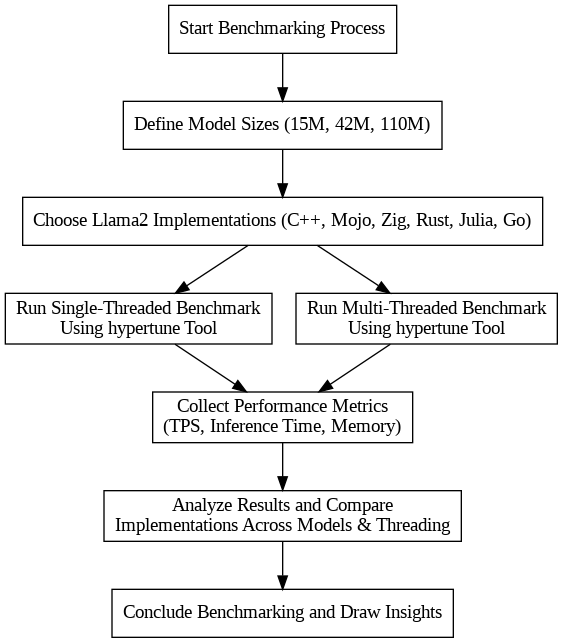
\includegraphics[width=\linewidth]{benchmark_flowchart_detailed}
  \caption{Benchmarking Process for Evaluating Llama2 Implementations across Model Sizes and Threading Configurations.}
\end{figure}

The flowchart (Figure 1) outlines a benchmarking process for evaluating different implementations of the Llama2 system across various model sizes and threading configurations. It starts by defining model sizes and selecting implementations in other programming languages. Then, it splits into two paths to run single-threaded and multi-threaded benchmarks using the hypertune tool. After collecting performance metrics like TPS, inference time, and memory usage, the results are analyzed to compare implementations across models and threading. Finally, insights are drawn from the analysis to conclude the benchmarking process.


\subsection{Testing Environment and Hardware}
The benchmarking was carried out on a MacBook Pro outfitted with an Apple M2 Max SoC, boasting a 10-core CPU, a 32-core GPU, and a 16-core Neural Engine. This hardware setup provides a robust and pertinent environment for assessing LLM inference performance on Apple Silicon. All tests were conducted solely in CPU-only mode to ensure consistency and isolate the performance of the language implementations.

\subsection{Benchmarking Framework and Tools}
To ensure reliable and comparable performance measurements, we implemented a custom benchmarking framework designed to execute LLM inference tasks consistently across all language implementations. We utilized the “Hypertune” tool, a fork of the popular hyperfine command-line benchmarking utility, with enhanced features for granular performance data capture. This allowed us to measure and record key metrics, including tokens per second, time per inference, and memory usage.


\subsection{Performance Metrics}
Two fundamental performance metrics were employed to assess the efficacy of LLM implementations: tokens per second and time per inference. Tokens per second quantifies the processing speed, reflecting the model's throughput, while time per inference measures the average duration for completing a single inference step, indicative of responsiveness and latency.

\subsection{Testing Process}
\subsubsection{Single-Threaded and Multi-Threaded Configurations: }
Each language implementation underwent testing in both single-threaded and multi-threaded configurations, where feasible, to assess its scalability and efficiency in leveraging available CPU cores. Multi-threaded tests were conducted with varying thread counts to explore the impact of parallel processing on performance.

\subsubsection{Model Conversion: }
To ensure equitable comparison across implementations, the Llama2 models were converted to the fp32 GGUF format utilizing the llama.cpp converter tool. This step was imperative to accommodate potential differences in model format requirements across implementations. Subsequently, each implementation loaded and executed the converted models for benchmarking purposes.

\subsubsection{Inference Execution: }
A series of inference tasks were executed using each implementation and model combination, with performance metrics recorded for subsequent analysis. These inference tasks involved presenting prompts and generating text completions, mirroring real-world LLM usage scenarios. Collected results were meticulously analyzed to discern and compare the performance characteristics of each implementation.

\subsection{Data Collection and Analysis}
The amassed performance data underwent rigorous scrutiny, employing statistical techniques and visualization tools to uncover nuanced insights. Through comparative analysis, trends in performance across different implementations were elucidated, allowing for a comprehensive evaluation of their strengths and weaknesses. By juxtaposing the performance of Mojo SDK with other established implementations, the study sought to highlight its comparative advantages and potential areas for improvement. The findings of this analysis served as the basis for drawing meaningful conclusions regarding the efficacy and suitability of Mojo SDK for LLM inference tasks on Apple Silicon.
\begin{figure}[htbp]
  \centering
  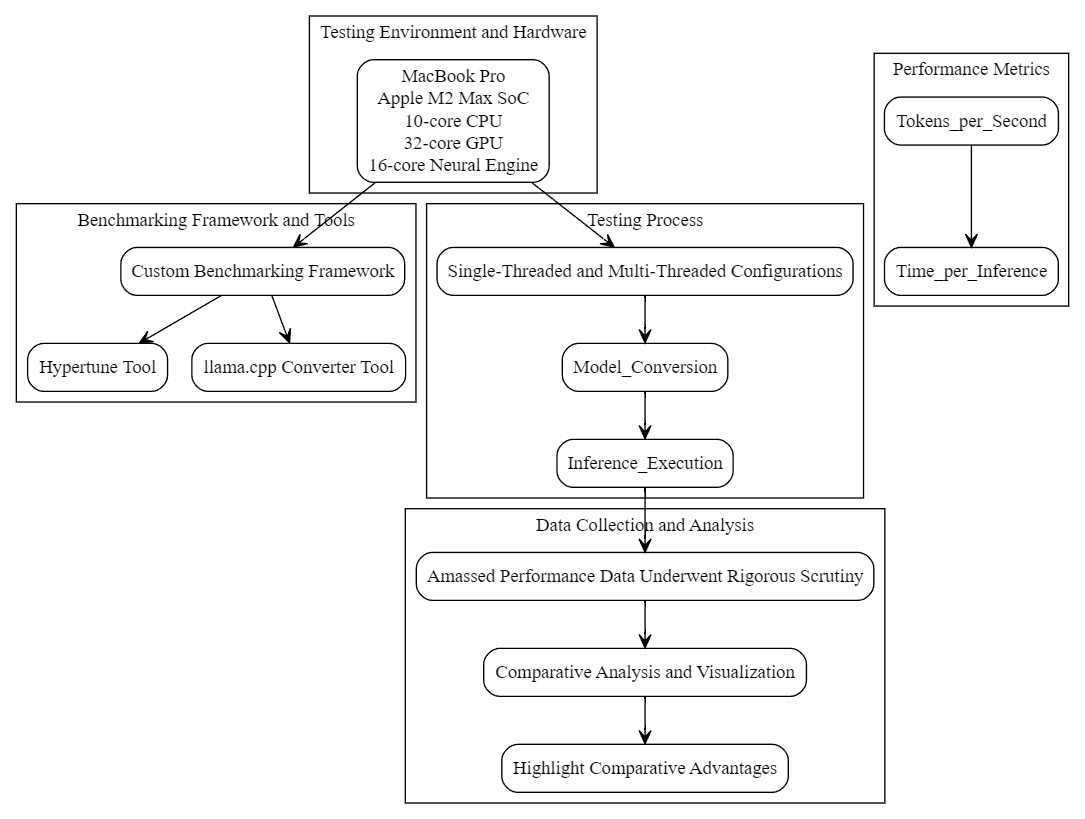
\includegraphics[width=\linewidth]{Figure_2}
  \caption{Overview Process for Evaluating LLM Implementations}
\end{figure}

\section{Results and Discussion}
The performance evaluation of LLM implementations (Figure 3) provides crucial insights into their efficiency and suitability for various tasks. By assessing metrics such as throughput, latency, and resource utilization across different languages and frameworks, researchers can identify optimal solutions for LLM inference, informing developers and researchers about the most effective approaches for their applications.
\begin{figure}[htbp]
  \centering
  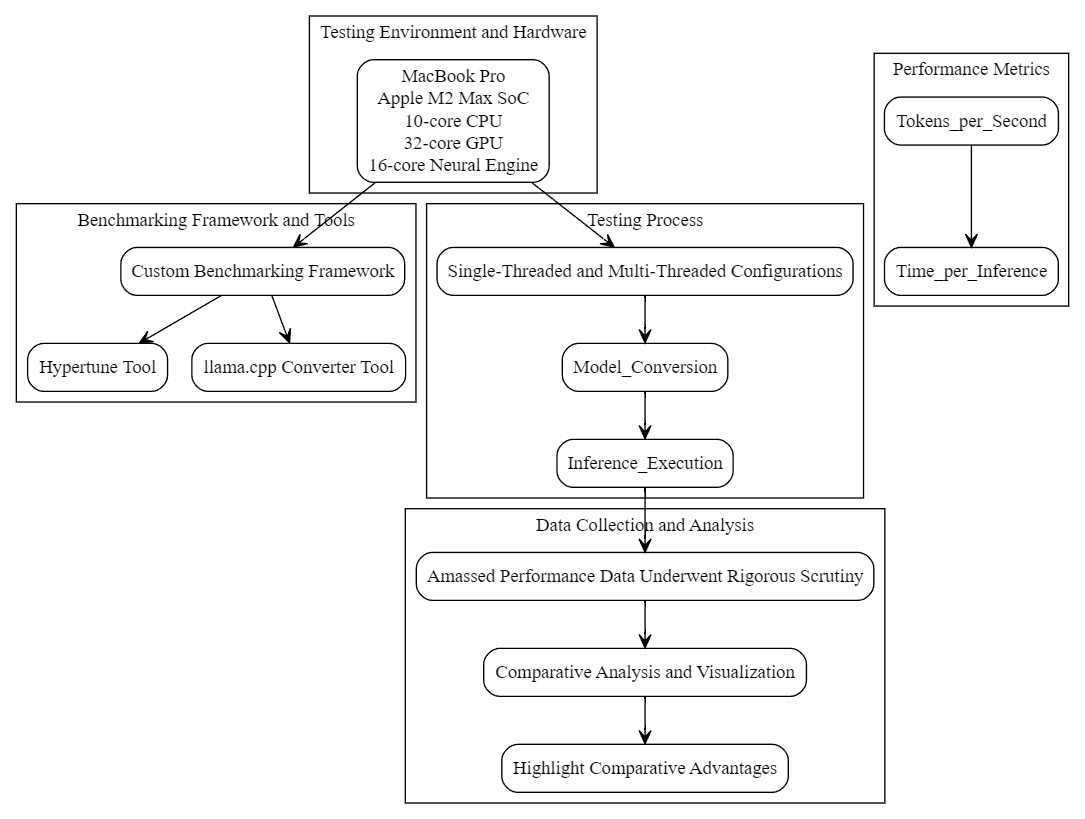
\includegraphics[width=\linewidth]{Figure_2}
  \caption{Performance Evaluation of LLM Implementations}
\end{figure}

\subsection{Multi-Threaded Performance Comparison}
The multi-threaded benchmarks conducted by the authors provide valuable insights into the performance of Mojo SDK and other language implementations for Llama2 inference. Key findings include:
\begin{itemize}
  \item Mojo SDK consistently demonstrates competitive performance across all model sizes, indicating its effectiveness regarding tokens per second and inference time. While not always the top performer, Mojo's Python-like usability and low-level optimization combination contribute to efficient LLM inference. Moreover, Mojo scales well with larger models, narrowing the performance gap with other implementations.
  \item C++ and Zig implementations exhibit strong performance, which is particularly noticeable in larger models. This underscores their suitability for computationally intensive tasks and effective utilization of modern hardware capabilities.
  \item Go, Rust, and Julia perform moderately, offering reasonable efficiency for LLM inference tasks. Additional optimizations and platform-specific tuning could further enhance their performance.
\end{itemize}


\begin{figure}[htbp]
  \centering
  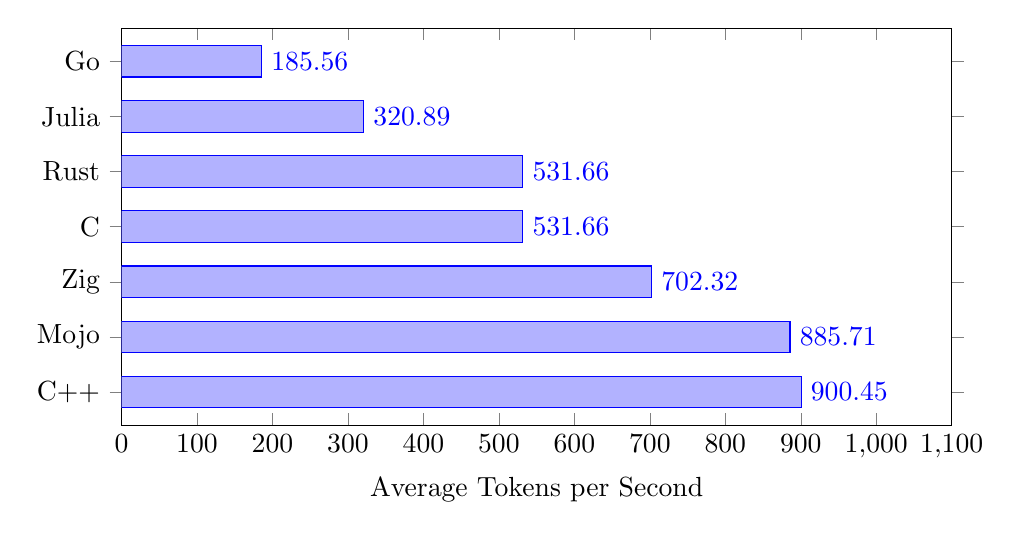
\begin{tikzpicture}
      \begin{axis}[
          y=0.7cm,
          bar width=0.4cm,
          width=\linewidth,
          height=8cm,
          symbolic y coords={C++, Mojo, Zig, C, Rust, Julia, Go},
          ytick=data,
          xbar,
          xlabel={Average Tokens per Second},
          nodes near coords,
          nodes near coords align={horizontal},
          xmin=0, % minimum value for x-axis
          xmax=1100,
          ]
          \addplot coordinates {(900.4463,C++) (885.71,Mojo) (702.3167,Zig) (531.6647,C) (531.6647,Rust) (320.887,Julia) (185.5577,Go)};
      \end{axis}
  \end{tikzpicture}
  \caption{Average Tokens per Second for stories15M.bin model}
\end{figure}

\begin{figure}[htbp]
  \centering
  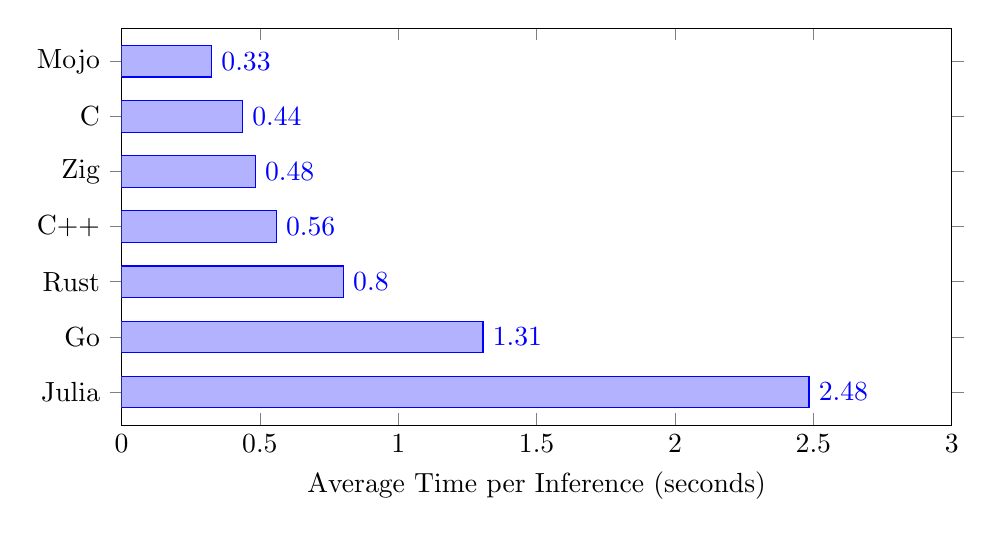
\begin{tikzpicture}
      \begin{axis}[
          y=0.7cm,
          bar width=0.4cm,
          width=\linewidth,
          height=8cm,
          symbolic y coords={Julia, Go, Rust, C++, Zig, C, Mojo},
          ytick=data,
          xbar,
          xlabel={Average Time per Inference (seconds)},
          nodes near coords,
          nodes near coords align={horizontal},
          xmin=0, % minimum value for x-axis
          xmax=3,
          ]
          \addplot coordinates {(2.48412,Julia) (1.306325,Go) (0.802,Rust) (0.5592776,C++) (0.4834227,Zig) (0.4373009,C) (0.325698,Mojo)};
      \end{axis}
  \end{tikzpicture}
  \caption{Average Time per Inference for stories15M.bin model}
\end{figure}

\begin{figure}[htbp]
  \centering
  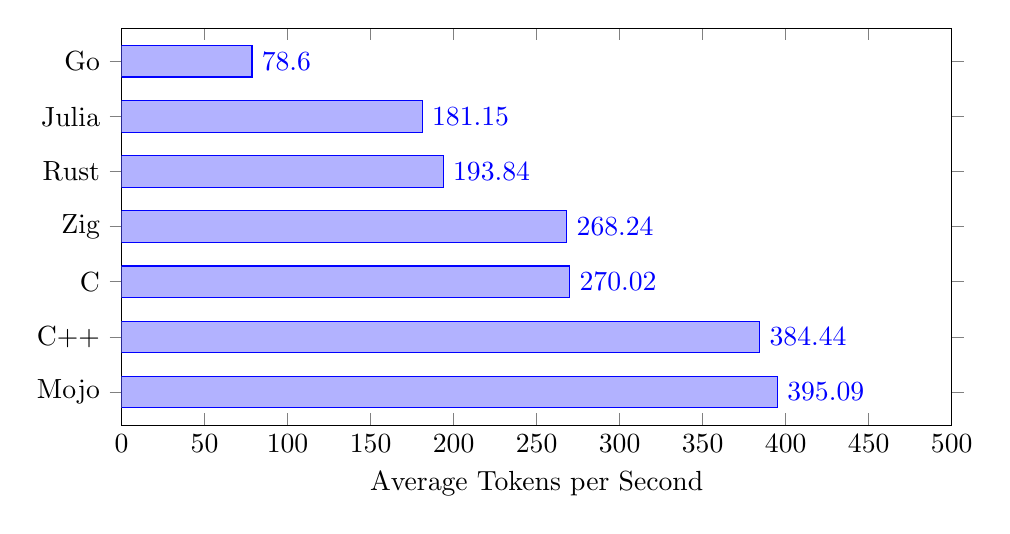
\begin{tikzpicture}
      \begin{axis}[
          y=0.7cm,
          bar width=0.4cm,
          width=\linewidth,
          height=8cm,
          symbolic y coords={Mojo, C++, C, Zig, Rust, Julia, Go},
          ytick=data,
          xbar,
          xlabel={Average Tokens per Second},
          nodes near coords,
          nodes near coords align={horizontal},
          xmin=0, % minimum value for x-axis
          xmax=500,
          ]
          \addplot coordinates {(395.088,Mojo) (384.4397,C++) (270.0187,C) (268.2443,Zig) (193.8413,Rust) (181.1473,Julia) (78.60167,Go)};
      \end{axis}
  \end{tikzpicture}
  \caption{Average Tokens per Second for stories42M.bin model}
\end{figure}

\begin{figure}[htbp]
  \centering
  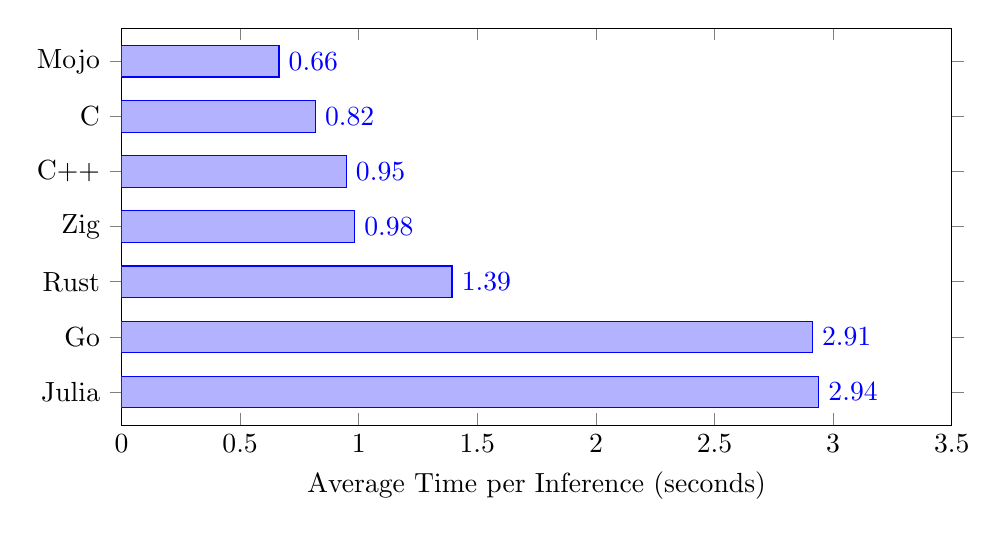
\begin{tikzpicture}
      \begin{axis}[
          y=0.7cm,
          bar width=0.4cm,
          width=\linewidth,
          height=8cm,
          symbolic y coords={Julia, Go, Rust, Zig, C++, C, Mojo},
          ytick=data,
          xbar,
          xlabel={Average Time per Inference (seconds)},
          nodes near coords,
          nodes near coords align={horizontal},
          xmin=0, % minimum value for x-axis
          xmax=3.5,
          ]
          \addplot coordinates {(2.939204,Julia) (2.912359,Go) (1.393408,Rust) (0.982617,Zig) (0.9472967,C++) (0.8171151,C) (0.6637589,Mojo)};
      \end{axis}
  \end{tikzpicture}
  \caption{Average Time per Inference for stories42M.bin model}
\end{figure}

\begin{figure}[htbp]
  \centering
  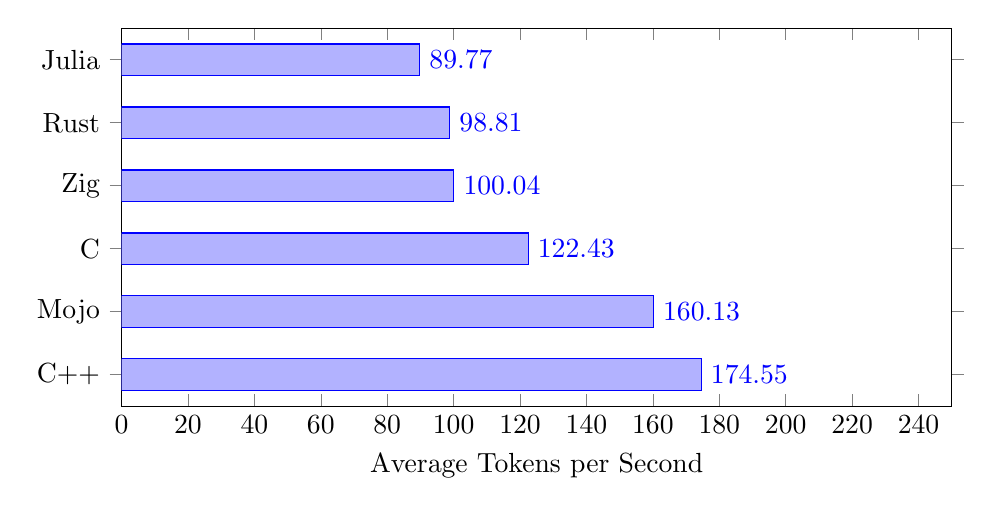
\begin{tikzpicture}
      \begin{axis}[
          y=0.8cm,
          bar width=0.4cm,
          width=\linewidth,
          height=8cm,
          symbolic y coords={C++, Mojo, C, Zig, Rust, Julia},
          ytick=data,
          xbar,
          xlabel={Average Tokens per Second},
          nodes near coords,
          nodes near coords align={horizontal},
          xmin=0, % minimum value for x-axis
          xmax=250,
          ]
          \addplot coordinates {(174.5473,C++) (160.132,Mojo) (122.4277,C) (100.0353,Zig) (98.8087,Rust) (89.77033,Julia)};
      \end{axis}
  \end{tikzpicture}
  \caption{Average Tokens per Second for stories110M.bin model}
\end{figure}

\begin{figure}[htbp]
  \centering
  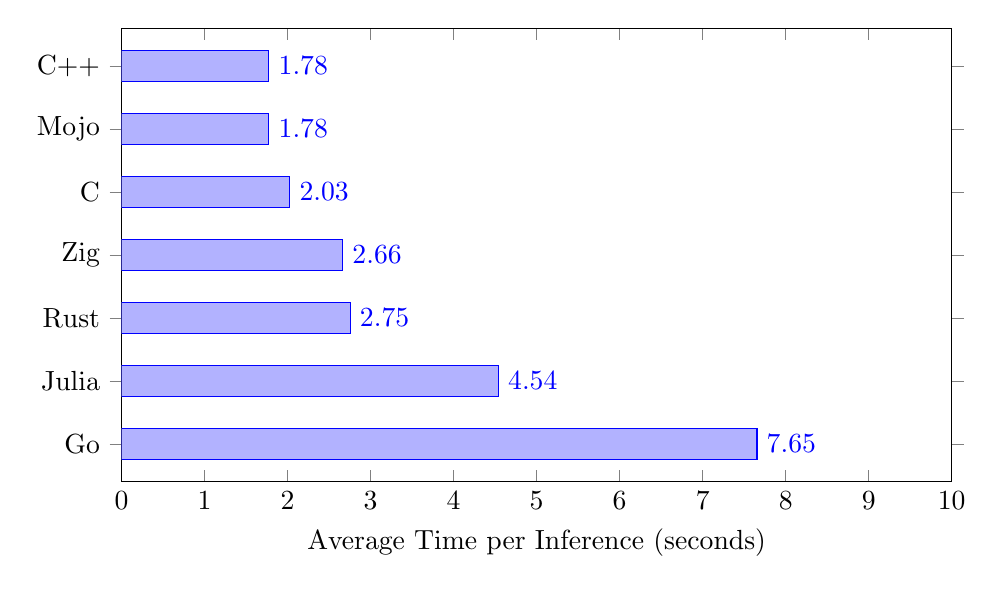
\begin{tikzpicture}
      \begin{axis}[
          y=0.8cm,
          bar width=0.4cm,
          width=\linewidth,
          height=8cm,
          symbolic y coords={Go, Julia, Rust, Zig, C, Mojo, C++},
          ytick=data,
          xbar,
          xmin=0, xmax=25,
          xlabel={Average Time per Inference (seconds)},
          nodes near coords,
          nodes near coords align={horizontal},
          xmin=0, % minimum value for x-axis
          xmax=10,
          ]
          \addplot coordinates {(7.653778,Go) (4.540055,Julia) (2.754481,Rust) (2.664162,Zig) (2.02678,C) (1.775346,Mojo) (1.775346,C++)};
      \end{axis}
  \end{tikzpicture}
  \caption{Average Time per Inference for stories110M.bin model.}
\end{figure}


\begin{itemize}

\item	Mojo SDK consistently demonstrates competitive performance across all model sizes, indicating its effectiveness regarding tokens per second and inference time. While not always the top performer, Mojo's Python-like usability and low-level optimization combination contribute to efficient LLM inference. Moreover, Mojo scales well with larger models, narrowing the performance gap with other implementations.

\item C++ and Zig implementations exhibit strong performance, which is particularly noticeable in larger models. This underscores their suitability for computationally intensive tasks and effective utilization of modern hardware capabilities.

\item	Go, Rust, and Julia perform moderately, offering reasonable efficiency for LLM inference tasks. Additional optimizations and platform-specific tuning could further enhance their performance.

\end{itemize}

\subsection{Single-Threaded Performance Comparison}
Single-threaded benchmarks provide a valuable perspective on the inherent efficiency of each implementation, independent of multi-threading capabilities. The results are summarized below:

\begin{figure}[htbp]
  \centering
  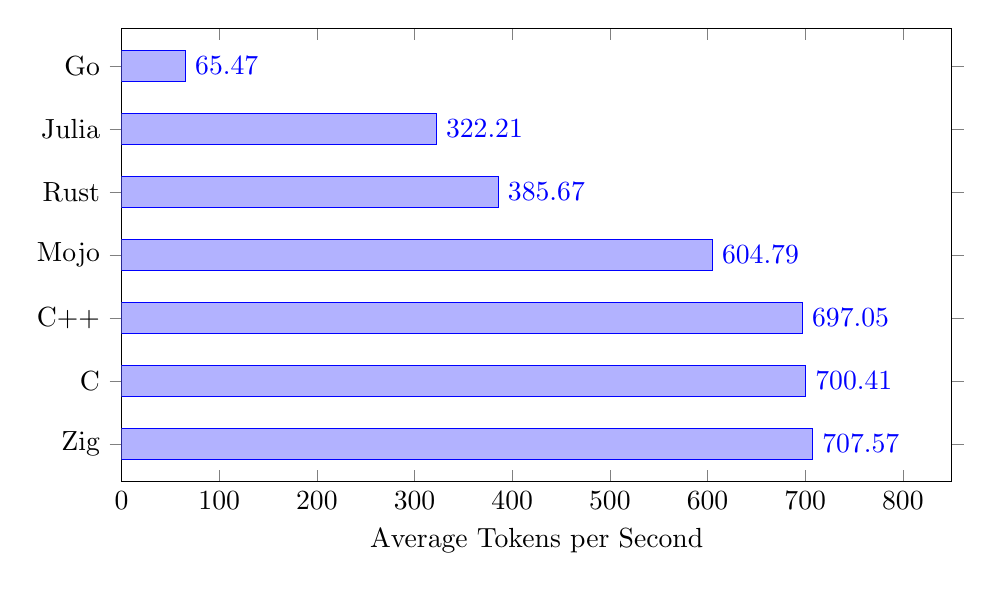
\begin{tikzpicture}
      \begin{axis}[
          y=0.8cm,
          bar width=0.4cm,
          width=\linewidth,
          height=8cm,
          symbolic y coords={Zig, C, C++, Mojo, Rust, Julia, Go},
          ytick=data,
          xbar,
          xlabel={Average Tokens per Second},
          nodes near coords,
          nodes near coords align={horizontal},
          xmin=0, % minimum value for x-axis
          xmax=850,
          ]
          \addplot coordinates {(707.5707,Zig) (700.4067,C) (697.0493,C++) (604.7863,Mojo) (385.6671,Rust) (322.2083,Julia) (65.466,Go)};
      \end{axis}
  \end{tikzpicture}
  \caption{Average Tokens per Second for stories15M.bin model}
\end{figure}

\begin{figure}[htbp]
  \centering
  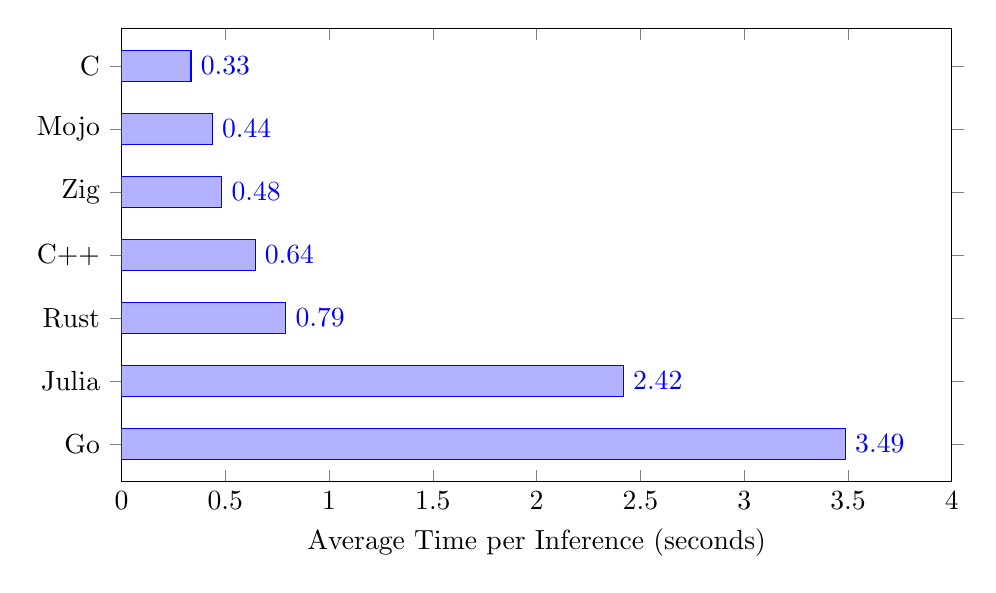
\begin{tikzpicture}
      \begin{axis}[
          y=0.8cm,
          bar width=0.4cm,
          width=\linewidth,
          height=8cm,
          symbolic y coords={Go, Julia, Rust, C++, Zig, Mojo, C},
          ytick=data,
          xbar,
          xlabel={Average Time per Inference (seconds)},
          nodes near coords,
          nodes near coords align={horizontal},
          xmin=0, % minimum value for x-axis
          xmax=4,
          ]
          \addplot coordinates {(3.487985,Go) (2.418289,Julia) (0.7912604,Rust) (0.6434277,C++) (0.4833996,Zig) (0.4374733,Mojo) (0.334866,C)};
      \end{axis}
  \end{tikzpicture}
  \caption{Average Time per Inference for stories15M.bin model}
\end{figure}

\begin{figure}[htbp]
  \centering
  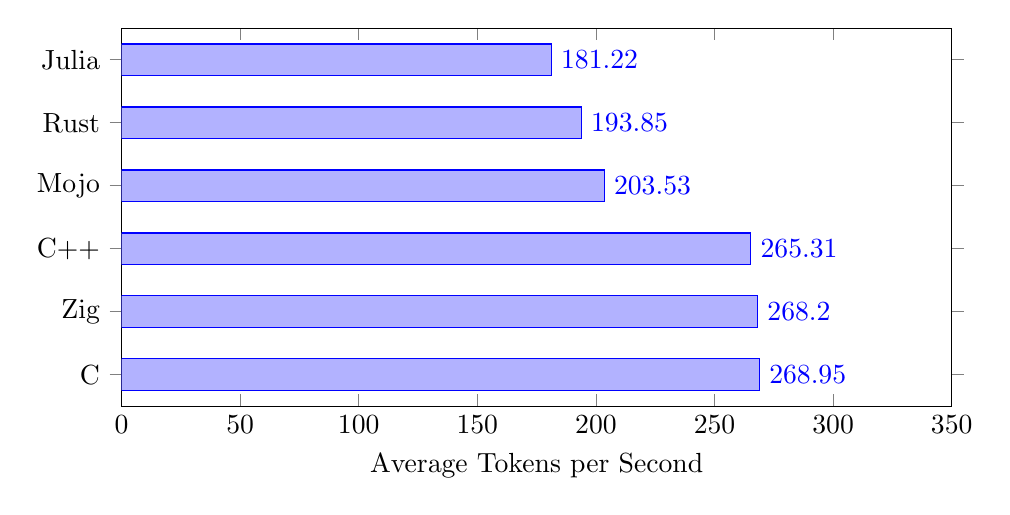
\begin{tikzpicture}
      \begin{axis}[
          y=0.8cm,
          bar width=0.4cm,
          width=\linewidth,
          height=8cm,
          symbolic y coords={C, Zig, C++, Mojo, Rust, Julia},
          ytick=data,
          xbar,
          xlabel={Average Tokens per Second},
          nodes near coords,
          nodes near coords align={horizontal},
          xmin=0, % minimum value for x-axis
          xmax=350,
          ]
          \addplot coordinates {(268.9483,C) (268.1983,Zig) (265.3133,C++) (203.529,Mojo) (193.8467,Rust) (181.22,Julia)};
      \end{axis}
  \end{tikzpicture}
  \caption{Average Tokens per Second for stories42M.bin model}
\end{figure}

\begin{figure}[htbp]
  \centering
  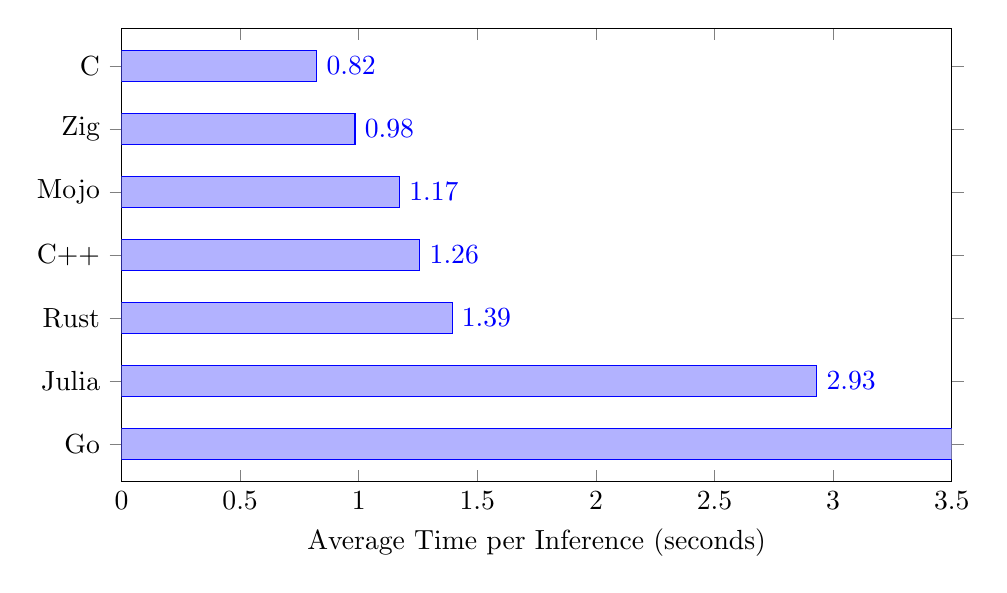
\begin{tikzpicture}
      \begin{axis}[
          y=0.8cm,
          bar width=0.4cm,
          width=\linewidth,
          height=8cm,
          symbolic y coords={Go, Julia, Rust, C++, Mojo, Zig, C},
          ytick=data,
          xbar,
          xlabel={Average Time per Inference (seconds)},
          nodes near coords,
          nodes near coords align={horizontal},
          xmin=0, % minimum value for x-axis
          xmax=3.5,
          ]
          \addplot coordinates {(8.589452,Go) (2.930905,Julia) (1.393492,Rust) (1.258079,C++) (1.172187,Mojo) (0.984326,Zig) (0.8232438,C)};
      \end{axis}
  \end{tikzpicture}
  \caption{Average Time per Inference  for stories42M.bin model}
\end{figure}

\begin{figure}[htbp]
  \centering
  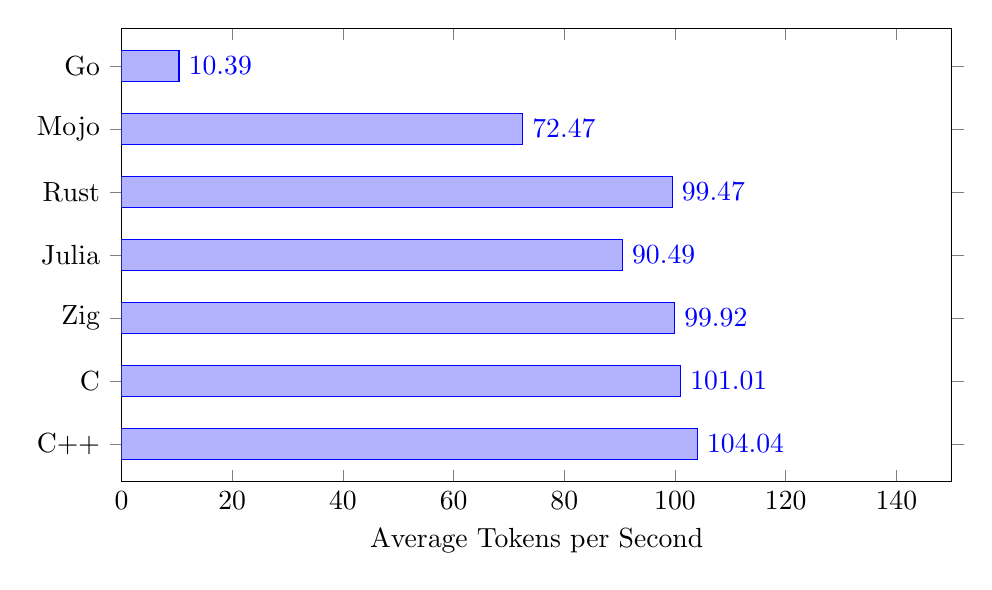
\begin{tikzpicture}
      \begin{axis}[
          y=0.8cm,
          bar width=0.4cm,
          width=\linewidth,
          height=8cm,
          symbolic y coords={C++, C, Zig, Julia, Rust, Mojo, Go},
          ytick=data,
          xbar,
          xlabel={Average Tokens per Second},
          nodes near coords,
          nodes near coords align={horizontal},
          xmin=0, % minimum value for x-axis
          xmax=150,
          ]
          \addplot coordinates {(104.0357,C++) (101.0133,C) (99.915,Zig) (90.48933,Julia) (99.4693,Rust) (72.46933,Mojo) (10.39367,Go)};
      \end{axis}
  \end{tikzpicture}
  \caption{Average Tokens per Second for stories110M.bin model}
\end{figure}

\begin{figure}[htbp]
  \centering
  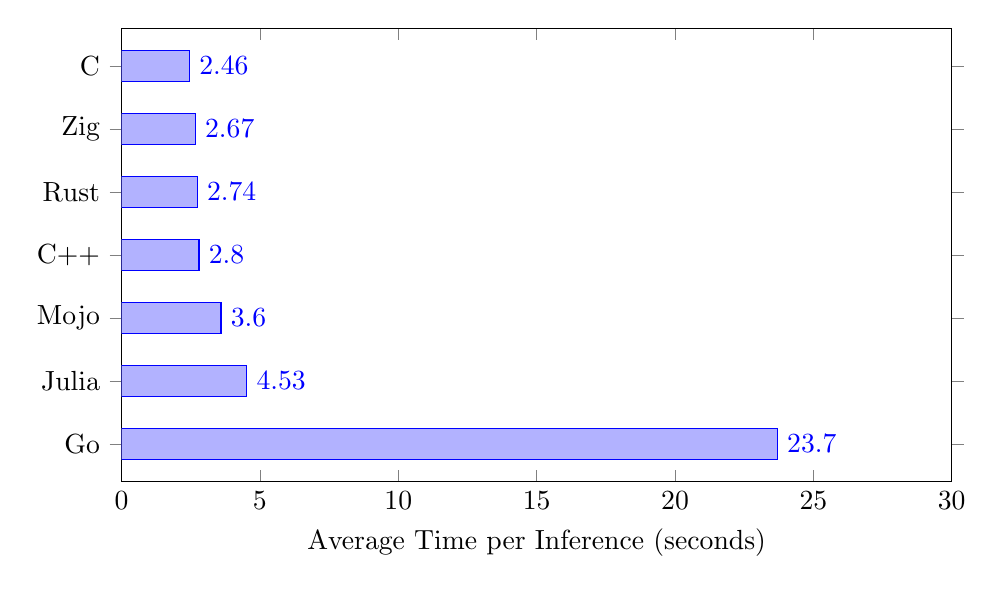
\begin{tikzpicture}
      \begin{axis}[
          y=0.8cm,
          bar width=0.4cm,
          width=\linewidth,
          height=8cm,
          symbolic y coords={Go, Julia, Mojo, C++, Rust, Zig, C},
          ytick=data,
          xbar,
          xlabel={Average Time per Inference (seconds)},
          nodes near coords,
          nodes near coords align={horizontal},
          xmin=0, % minimum value for x-axis
          xmax=30, % maximum value for x-axis
          ]
          \addplot coordinates {(23.69974,Go) (4.52782,Julia) (3.595333,Mojo) (2.799485,C++) (2.738403,Rust) (2.668282,Zig) (2.4586,C)};
      \end{axis}
  \end{tikzpicture}
  \caption{Average Time per Inference for stories110M.bin model}
\end{figure}

\begin{itemize}

\item C implementations excel in single-threaded scenarios with the llama2.c implementation consistently achieves high tokens per second and low inference times across all model sizes. This highlights C's effectiveness for highly optimized, single-threaded tasks.

\item Mojo SDK maintains single-threaded solid performance, surpassing several other implementations while not matching the speed of C. This underscores the efficiency of Mojo's design and compilation strategy.

\item Zig consistently performs consistently across single-threaded and multi-threaded configurations, suggesting efficient core logic and minimal overhead threading.

\end{itemize}

The results affirm Mojo SDK as a compelling choice for Llama2 inference on Apple Silicon, offering competitive performance with optimized implementations in C and C++, alongside greater ease of use and compatibility with the Python ecosystem. However, performance may vary based on hardware configurations, model sizes, and inference tasks. Further optimization and platform-specific tuning can enhance performance across all implementations, including Mojo SDK.
The benchmarking results underscore Mojo SDK's effectiveness as an efficient solution for Llama2 inference on Apple Silicon. Its competitive performance, ease of use, and Python compatibility present a unique advantage in the LLM deployment landscape. Leveraging the extensive Python ecosystem for pre-processing, post-processing, and integration with other machine-learning tools enhances Mojo's appeal to developers seeking performance and productivity.


\subsection{Advantages of Mojo SDK}
Mojo SDK streamlines LLM development with its Python-like syntax and seamless Python library integration, simplifying complexities inherent in lower-level languages like C or C++. This abstraction lets developers focus on model integration and application logic rather than grapple with memory management or performance optimization intricacies. Despite its high-level approach, Mojo's compiler infrastructure ensures optimal performance, often rivaling or surpassing established implementations. Its accessibility to Python developers broadens its user base, while an active community fosters collaboration and accelerates technology adoption.


\subsection{Limitations and Future Work}
While this study focused on CPU-based inference on Apple Silicon, future research could explore the impact of GPU acceleration on performance, particularly considering Mojo's adaptability to diverse hardware. Additionally, investigating Mojo SDK's performance and optimization across different hardware platforms with varying architectures or resource constraints would enhance understanding its capabilities and limitations.
Moreover, the emergence of efficient and user-friendly LLM inference solutions like Mojo SDK has significant implications for the future of LLM deployment. Lowering the barrier to entry and enabling efficient execution on resource-constrained devices, Mojo empowers a broader range of developers and researchers to explore the potential of LLMs in various applications. This could lead to accelerated innovation in edge computing, personalized AI assistants, and LLM-powered mobile applications.


\section{Conclusion}
In conclusion, this study highlights Mojo SDK as a compelling solution for efficient and accessible Llama2 inference on Apple Silicon. Its competitive performance, ease of use, and Python compatibility position it as a valuable tool for developers and researchers alike. By simplifying development processes and enabling efficient execution on resource-constrained devices, Mojo SDK has the potential to democratize access to powerful language models, fostering innovation across various domains.
Looking ahead, further exploration of Mojo's capabilities with GPU acceleration, diverse hardware platforms, and evolving LLM architectures holds promise for the future of LLM deployment. As the LLM landscape evolves, Mojo SDK emerges as a promising framework that empowers a broader range of users to harness the power of LLMs and unlock their transformative potential, driving innovation and advancements in the field.





\citestyle{acmauthoryear}



% Add more \cite commands as needed for other references

\bibliographystyle{ACM-Reference-Format} % Choose your bibliography style
\bibliography{sample-base} % Name of your BibTeX file without the extension


\end{document}
\endinput
%%
%% End of file `sample-sigconf.tex'.
